\subsection*{Resultados Empíricos - Insertion Sort}

\qquad Os testes experimentais foram executados com vetores de tamanhos variando de $n = 10$ a $n = 1.000.000$ elementos, sob três configurações de entrada: crescente (melhor caso), decrescente (pior caso) e aleatória (caso médio). A Tabela \ref{tab:insertion_tempos} apresenta a compilação dos tempos de execução aferidos em segundos.

\begin{table}[htbp]
    \centering
    \caption{Tempo de execução (em segundos) do Insertion Sort para diferentes tamanhos de entrada.}
    \label{tab:insertion_tempos}
    \vspace{0.2cm}
    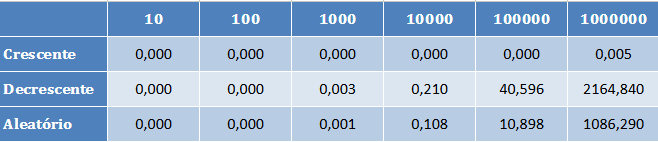
\includegraphics[width=0.9\textwidth]{Imagens/Insertion Sort/tabela insertion.png}
\end{table}

\qquad A representação gráfica do desempenho do algoritmo é ilustrada na Figura \ref{fig:insertion_grafico}. A curva observada valida diretamente a modelagem matemática assintótica desenvolvida nas seções anteriores.

\begin{figure}[htbp]
    \centering
    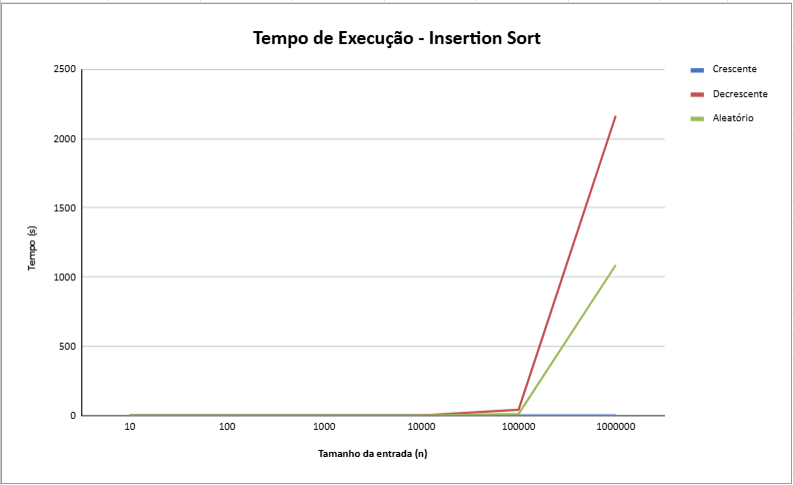
\includegraphics[width=0.85\textwidth]{Imagens/Insertion Sort/grafico insertion.png}
    \caption{Curvas de desempenho do Insertion Sort em função da ordenação e do tamanho da entrada ($n$).}
    \label{fig:insertion_grafico}
\end{figure}

\qquad A interpretação dos dados experimentais evidencia os seguintes padrões operacionais:

\begin{itemize}
    \item \textbf{Cenário Crescente (Melhor Caso):} O tempo de execução permaneceu inexpressivo até a escala de $1.000.000$ elementos (0,005 s), comprovando a eficiência do comportamento linear $O(n)$, decorrente da ausência de trocas internas no vetor.
    \item \textbf{Cenário Decrescente (Pior Caso):} Demonstra a inflexão característica da complexidade quadrática $O(n^2)$. O tempo eleva-se de 40,59 s ($n = 100.000$) para 2164,84 s ($\approx 36$ minutos para $n = 1.000.000$), consequência do custo máximo de comparações e deslocamentos a cada inserção.
    \item \textbf{Cenário Aleatório (Caso Médio):} O tempo registrado para $n = 1.000.000$ (1086,29 s) é aproximadamente metade do valor medido no pior caso. Esse resultado valida empiricamente o modelo matemático de constantes operacionais $T(n) \approx \frac{1}{2} T_{pior}(n)$, preservando a assíntota $O(n^2)$.
\end{itemize}